\section{Compilers \weekDoran{2}}
	\subsection{Translation Process}
	
		\begin{table}[H]\centering
			\begin{tabular}{p{0.425\linewidth}p{0.425\linewidth}}
				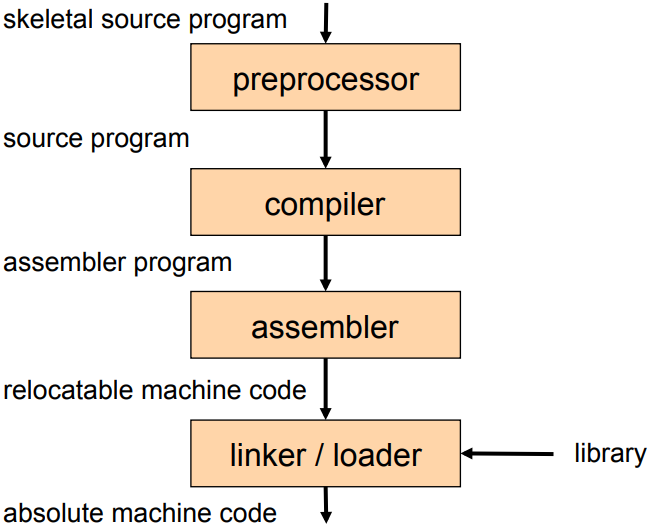
\includegraphics[scale=0.4]{./pictures/translation.png}
					& 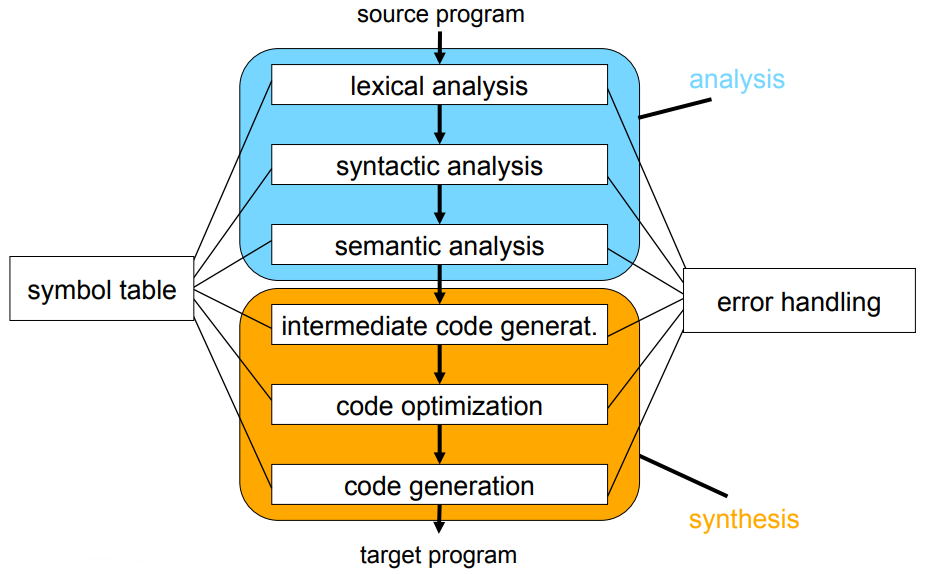
\includegraphics[scale=0.4]{./pictures/analysisSynthesis.png}\\
			\end{tabular}
		\end{table}

		\begin{longtable}{|>{\bfseries}p{0.2\linewidth}|p{0.75\linewidth}|}
			\hline
			Lexical Analysis
				& Scanning the programme and splitting into symbols.\\
			\hline
			Syntactic Analysis
				& Parsing symbol sequences and construction of sentences.\newline
				sentences are described by a context-free grammar.\\
			\hline
			Semantic Analysis
				& Make sure the program parts "reasonably" fit together, eg. type casts.\\
			\hline
			Intermediate Code
				& Machine independent \textrightarrow\ simplified retargeting.\\
			\hline
			Optimisation
				& Both intermediate and target code can be optimized.\\
			\hline
		\end{longtable}
			